\documentclass[a4paper,12pt]{report}

\usepackage{alltt, fancyvrb, url}
\usepackage{graphicx}
\usepackage[utf8]{inputenc}
\usepackage{float}
\usepackage{hyperref}

% Questo commentalo se vuoi scrivere in inglese.
\usepackage[italian]{babel}

\usepackage[italian]{cleveref}

\title{Relario: Tales of Relano\\Progetto per il corso di\\``Programmazione ad Oggetti''}

\author{Lorenzo Cinelli, Mihai Mazuru, Kimi Osti, Sara Panfini}
\date{\today}


\begin{document}

\maketitle

\tableofcontents

\chapter{Analisi}


\section{Descrizione e requisiti}

Il software realizzato è un videogioco 2D con vista dall’alto. Il suo svolgimento gira attorno a un personaggio principale, controllato dall’utente, che deve attraversare le stanze di un castello per raggiungere lo scontro finale con il Re, di cui deve conquistare il trono.
%
\newline Durante l’esplorazione delle stanze all’utente potranno essere affidate delle quest da completare per poter procedere correttamente.
%
\newline Inoltre, gli verranno presentato delle stanze quasi completamente interattive. In particolare, ci saranno dei personaggi non giocanti (neutri, alleati o nemici) che potranno, al momento dell’interazione, mostrare un messaggio, donare degli oggetti oppure ingaggiare un combattimento. Inoltre, sarà possibile interagire con gran parte degli elementi di arredo presenti in stanza, tra cui elementi come armature o vasi contenenti oggetti collezionabili oppure tappeti o botole che possono celare al loro interno nemici.
%
\newline Il combattimento si svolge per turni. Ad ogni turno, il giocatore può decidere se attaccare o chiedere pietà al nemico, così come può navigare il suo inventario e usare oggetti senza perdere il diritto al turno. Il nemico, in caso venga chiesta pietà, potrebbe concederla oppure rifiutarla e attaccare immediatamente il giocatore. 

\subsubsection{Requisiti funzionali}
\begin{itemize}
	\item I nemici all'interno del gioco saranno di varie tipologie, e dovranno offrire un comportamento variabile all'utente per quanto riguarda le richieste di pietà;
	\item L'arredo delle stanze viene generato casualmente garantendo l'assenza di sovrapposizioni, e le diverse tipologie di elementi di arredo devono offrire diversi scenari di interazione;
	\item Le quest devono essere di diverse tipologie e richiedere diverse azioni da parte del giocatore;
	\item Il combattimento finale deve poter offrire una scelta al giocatore, che sarà in grado di avviare finali diversi.
\end{itemize}

\subsubsection{Requisiti non funzionali}
\begin{itemize}
	\item Per offire un'esperienza gradevole all'utente, si mira a realizzare un software efficiente.
	\item Il software sarà portabile su tutti i maggiori sistemi operativi.
\end{itemize}


\section{Modello del Dominio}

Il dominio applicativo dell’applicazione viene modellato in ogni momento dal concetto di stanza, ovvero il “container” all’interno di cui si svolge la fase centrale del gioco. All’interno della stanza, oltre al personaggio principale, si trovano altre entità, che possono essere personaggi viventi non giocanti (nemici o generici NPC) oppure elementi di arredo. Il giocatore può possedere nel suo inventario diversi oggetti, che vengono anch’essi modellati come entità. In questo scenario, diventa possibile gestire tramite la stanza e le informazioni che ogni entità offre l’intero modello del dominio, estraendo le istanze di interesse per gestire le situazioni contingenti come il combattimento. 
%
\newline Per quanto riguarda l’arredamento, le entità si dividono in tre tipologie fondamentali: arredamento interattivo, che blocca il movimento ma permette interazione, e può rilasciare un oggetto che il giocatore aggiungerà al proprio inventario al momento dell’interazione; arredamento calpestabile, che non ostruisce il movimento e permette interazione, ma può nascondere un nemico con cui viene avviato il combattimento non appena vi si interagisce; arredamento passivo, che ostacola il movimento e non permette alcun tipo di interazione. 
%
\newline Per quanto riguarda i nemici, ad ognuno viene associato un tipo, che ne definisce il livello di difficoltà. Quando viene sconfitto, un nemico rilascia un oggetto di inventario che il giocatore aggiungerà al proprio inventario al momento della vittoria. Ad ogni nemico viene poi associato un comportamento in caso di richieste di pietà, indipendente dal tipo e proprio di ogni singola istanza. In caso il giocatore venga risparmiato dal nemico, non ottiene il suo bottino.
%
\newline Gli NPC modellano tutti i personaggi non ostili all’interno del gioco, con cui sarà possibile interagire in ogni momento. Anche loro possono rilasciare oggetti di inventario al momento dell’interazione, oppure mostrare messaggi, che potranno o meno aiutare il giocatore a completare la quest.
%
\newline Il personaggio principale, che si muove nella mappa e interagisce con il resto delle entità presenti, può portare con sé alcuni oggetti di inventario ottenuti interagendo con le altre entità. Questi oggetti possono essere di vario tipo, e a seconda della tipologia offrire diversi effetti (cura, aumento del danno per le armi e protezione per le armature, oppure nessuno per gli oggetti collezionabili). Le armi e le armature, per essere effettive, devono essere equipaggiate, e hanno una durabilità limitata. Al momento dell’uso dell’oggetto, il suo effetto viene attivato sul giocatore. Un oggetto qualsiasi può anche essere scartato per liberare spazio nell’inventario, che ha capacità limitata.


\begin{figure}[H]
	\centering{}
	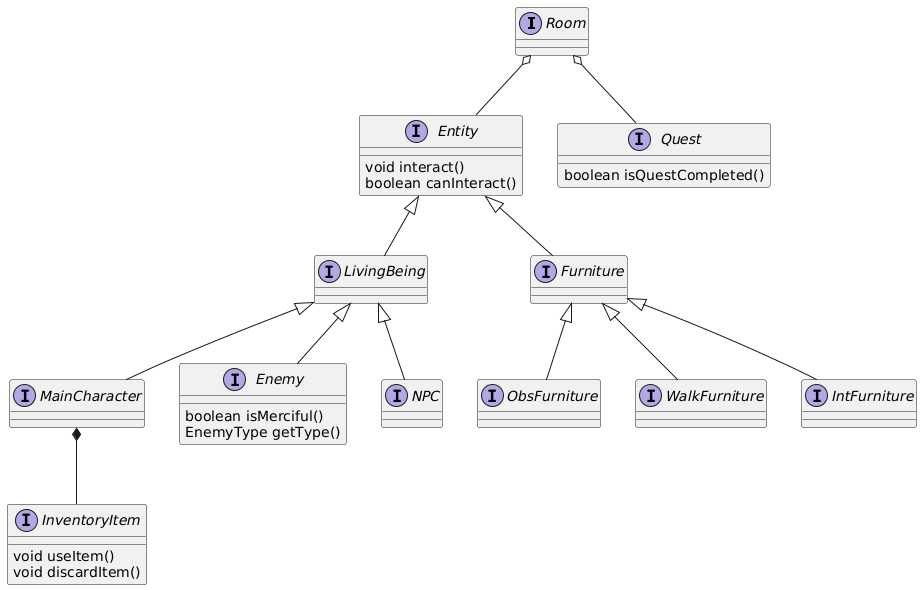
\includegraphics[width=\textwidth]{img/model.png}
	\caption{Schema UML del dominio applicativo}
	\label{img/model-image}
\end{figure}


\chapter{Design}

\section{Architettura}

Il software si basa sul modello architetturale di MVC, nella sua declinazione standard. In ogni fase
di gioco, quindi, la View sarà destinata a gestire le interazioni di Input/Output con l'utente, e segnalerà al
Controller il verificarsi di eventi dipendenti dall'utente (come la pressione di un tasto). Sarà quindi il Controller
a gestire il comportamento che deriva dagli eventi registrati dalla View, ed eventualmente a notificare al Model la
necessità di modificare il suo stato.
\newline Il Model, quindi, deve offrire almeno un entry point al Controller per ricevere i suoi messaggi. In particolare,
sapendo che il dominio applicativo prevede due momenti fondamentali di gioco (il combattimento e l'esplorazione) durante
cui vengono esposti aspetti molto diversi del dominio applicativo, è logico modellare qui due entry point che mappino
questa distinzione. In tale modo, un qualsiasi aspetto non modificabile durante una fase di gioco è completamente
nascosto rispetto all'esterno. 

\begin{figure}[H]
	\centering{}
	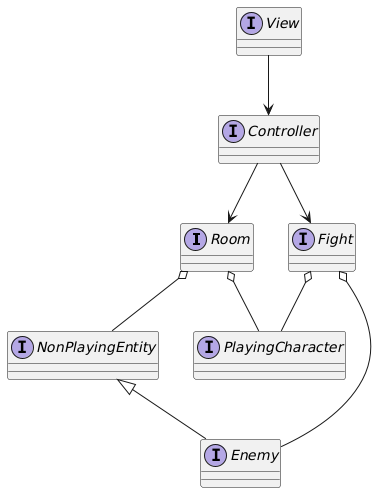
\includegraphics[width=\textwidth]{img/entryPoints.png}
	\caption{Schema UML degli entry point dei rapporti fra componenti di MVC}
	\label{img:entryPoints}
\end{figure}

Nell'immagine si evidenzia in particolare la direzionalità del rapporto fra Controller e Model. Ciò per sottolineare
ulteriormente come quest'ultimo rimanga in attesa di ricevere i messaggi del Controller per modificare il proprio stato,
in particolare offrendo due entry point che fanno da interfaccia a due sottoinsiemi del dominio applicativo
solo parzialmente sovrapposti. Questo è fondamentale in termini architetturali per preservare lo stato delle entità
del dominio, a cui non si può accedere a meno che non siano direttamente coinvolte nello scenario di gioco.
\newline Inoltre, si vede come la View offra un solo entry point che scambia messaggi con il Controller e che non viene
vista da nessun altro elemento dell'architettura. In particolare, strutturare in questo modo la View permette di
realizzarla con un elevato grado di indipendenza dal resto del sistema. In tale modo è possibile collegare al Controller
una qualsiasi interfaccia di Input/Output indipendentemente dalla sua tecnica implementativa, aumentando quindi
la mantenibilità e la modificabilità del software realizzato. 

\section{Design dettagliato}



\chapter{Sviluppo}
\section{Testing automatizzato}

Il testing automatizzato è un requisito di qualunque progetto software che si rispetti, e consente di verificare che non vi siano regressioni nelle funzionalità a fronte di aggiornamenti.
%
Per quanto riguarda questo progetto è considerato sufficiente un test minimale, a patto che sia completamente automatico.
%
Test che richiedono l'intervento da parte dell'utente sono considerati \textit{negativamente} nel computo del punteggio finale.

\subsection*{Elementi positivi}

\begin{itemize}
 \item Si descrivono molto brevemente i componenti che si è deciso di sottoporre a test automatizzato.
 \item Si utilizzano suite specifiche (e.g. JUnit) per il testing automatico.
\end{itemize}

\subsection*{Elementi negativi}
\begin{itemize}
 \item Non si realizza alcun test automatico.
 \item La non presenza di testing viene aggravata dall'adduzione di motivazioni non valide. Ad esempio, si scrive che l'interfaccia grafica non è testata automaticamente perché è \emph{impossibile} farlo\footnote{Testare in modo automatico le interfacce grafiche è possibile (si veda, come esempio, \url{https://github.com/TestFX/TestFX}), semplicemente nel corso non c'è modo e tempo di introdurvi questo livello di complessità. Il fatto che non vi sia stato insegnato come farlo non implica che sia impossibile!}.
 \item Si descrive un testing di tipo manuale in maniera prolissa.
 \item Si descrivono test effettuati manualmente che sarebbero potuti essere automatizzati, ad esempio scrivendo che si è usata l'applicazione manualmente.
 \item Si descrivono test non presenti nei sorgenti del progetto.
 \item I test, quando eseguiti, falliscono.
\end{itemize}

\section{Note di sviluppo}

Questa sezione, come quella riguardante il design dettagliato va svolta \textbf{singolarmente da ogni membro del gruppo}.
%
Nella prima parte, ciascuno dovrà mostrare degli esempi di codice particolarmente ben realizzati,
che dimostrino proefficienza con funzionalità avanzate del linguaggio e capacità di spingersi oltre le librerie mostrate a lezione.

\begin{itemize}
	\item \textbf{Elencare} (fare un semplice elenco per punti, non un testo!) le feature \textit{avanzate} del linguaggio e dell'ecosistema Java che sono state
utilizzate. Le feature di interesse sono:
	\begin{itemize}
		\item Progettazione con generici, ad esempio costruzione di nuovi tipi generici, e uso di generici bounded.
		L'uso di classi generiche di libreria non è considerato avanzato.
		\item Uso di lambda expressions
		\item Uso di \texttt{Stream}, di \texttt{Optional} o di altri costrutti funzionali
		\item Uso di reflection
		\item Definizione ed uso di nuove annotazioni
		\item Uso del Java Platform Module System
		\item Uso di parti della libreria JDK non spiegate a lezione (networking, compressione, parsing XML, eccetera...)
		\item Uso di librerie di terze parti (incluso JavaFX): Google Guava, Apache Commons...
	\end{itemize}
	\item Si faccia molta attenzione a non scrivere banalità, elencando qui features di tipo ``core'', come le eccezioni, le enumerazioni, o le inner class: nessuna di queste è considerata avanzata.
	\item Per ogni feature avanzata, mostrata, includere:
	\begin{itemize}
		\item Nome della feature
		\item Permalink GitHub al punto nel codice in cui è stata utilizzata
	\end{itemize}
\end{itemize}

In questa sezione, \textit{dopo l'elenco},
vanno menzionati ed attributi con precisione eventuali pezzi di codice ``riadattati'' (o scopiazzati...) da Internet o da altri progetti,
pratica che tolleriamo ma che non raccomandiamo.
%
Si rammenta agli studenti che non è consentito partire da progetti esistenti e procedere per modifiche successive.
%
Si ricorda anche che i docenti hanno in mano strumenti antiplagio piuttosto raffinati e che ``capiscono'' il codice e la storia delle modifiche del progetto,
per cui tecniche banali come cambiare nomi (di classi, metodi, campi, parametri, o variabili locali),
aggiungere o togliere commenti,
oppure riordinare i membri di una classe vengono individuate senza problemi.
%
Le regole del progetto spiegano in dettaglio l'approccio dei docenti verso atti gravi come il plagiarismo.

I pattern di design \textbf{non} vanno messi qui.
%
L'uso di pattern di design (come suggerisce il nome) è un aspetto avanzato di design, non di implementazione,
e non va in questa sezione.

\subsection*{Elementi positivi}

\begin{itemize}
	\item Si elencano gli aspetti avanzati di linguaggio che sono stati impiegati
	\item Si elencano le librerie che sono state utilizzate
	\item Per ciascun elemento, si fornisce un permalink
	\item Ogni permalink fa riferimento ad uno snippet di codice scritto dall'autore della sezione (i docenti verificheranno usando \texttt{git blame})
	\item Se si è utilizzato un particolare algoritmo, se ne cita la fonte originale.
	Ad esempio, se si è usato Mersenne Twister per la generazione di numeri pseudo-random, si cita \cite{mersenne}.
	\item Si identificano parti di codice prese da altri progetti, dal web, o comunque scritte in forma originale da altre persone.
	In tal senso, si ricorda che agli ingegneri non è richiesto di re-inventare la ruota continuamente:
	se si cita debitamente la sorgente è tollerato fare uso di di snippet di codice open source per risolvere velocemente problemi non banali.
	Nel caso in cui si usino snippet di codice di qualità discutibile,
	oltre a menzionarne l'autore originale si invitano gli studenti ad adeguare tali parti di codice agli standard e allo stile del progetto.
	Contestualmente, si fa presente che è largamente meglio fare uso di una libreria che copiarsi pezzi di codice:
	qualora vi sia scelta (e tipicamente c'è), si preferisca la prima via.
\end{itemize}

\subsection*{Elementi negativi}
\begin{itemize}
	\item Si elencano feature core del linguaggio invece di quelle segnalate. Esempi di feature core da non menzionare sono:
    \begin{itemize}
        \item eccezioni;
        \item classi innestate;
        \item enumerazioni;
        \item interfacce.
    \end{itemize}
	\item Si elencano applicazioni di terze parti (peggio se per usarle occorre licenza, e lo studente ne è sprovvisto) che non c'entrano nulla con lo sviluppo, ad esempio:
    \begin{itemize}
        \item Editor di grafica vettoriale come Inkscape o Adobe Illustrator;
        \item Editor di grafica scalare come GIMP o Adobe Photoshop;
        \item Editor di audio come Audacity;
        \item Strumenti di design dell'interfaccia grafica come SceneBuilder: il codice è in ogni caso inteso come sviluppato da voi.
    \end{itemize}
	\item Si descrivono aspetti di scarsa rilevanza, o si scende in dettagli inutili.
	\item Sono presenti parti di codice sviluppate originalmente da altri che non vengono debitamente segnalate.
	In tal senso, si ricorda agli studenti che i docenti hanno accesso a tutti i progetti degli anni passati,
	a Stack Overflow,
	ai principali blog di sviluppatori ed esperti Java,
	ai blog dedicati allo sviluppo di soluzioni e applicazioni
	(inclusi blog dedicati ad Android e allo sviluppo di videogame),
	nonché ai vari GitHub, GitLab, e Bitbucket.
	Conseguentemente, è \emph{molto} conveniente \emph{citare} una fonte ed usarla invece di tentare di spacciare per proprio il lavoro di altri.
	\item Si elencano design pattern
\end{itemize}

\subsection{Esempio}

\subsubsection{Utilizzo della libreria SLF4J}

Utilizzata in vari punti.
Un esempio è \url{https://github.com/AlchemistSimulator/Alchemist/blob/5c17f8b76920c78d955d478864ac1f11508ed9ad/alchemist-swingui/src/main/java/it/unibo/alchemist/boundary/swingui/effect/impl/EffectBuilder.java#L49}

\subsubsection{Utilizzo di \texttt{LoadingCache} dalla libreria Google Guava}

Permalink: \url{https://github.com/AlchemistSimulator/Alchemist/blob/d8a1799027d7d685569e15316a32e6394632ce71/alchemist-incarnation-protelis/src/main/java/it/unibo/alchemist/protelis/AlchemistExecutionContext.java#L141-L143}

\subsubsection{Utilizzo di \texttt{Stream} e lambda expressions}

Usate pervasivamente. Il seguente è un singolo esempio.
Permalink: \url{https://github.com/AlchemistSimulator/Alchemist/blob/d8a1799027d7d685569e15316a32e6394632ce71/alchemist-incarnation-protelis/src/main/java/it/unibo/alchemist/model/ProtelisIncarnation.java#L98-L120}

\subsubsection{Scrittura di metodo generico con parametri contravarianti}

Permalink: \url{https://github.com/AlchemistSimulator/Alchemist/blob/d8a1799027d7d685569e15316a32e6394632ce71/alchemist-incarnation-protelis/src/main/java/it/unibo/alchemist/protelis/AlchemistExecutionContext.java#L141-L143}

\subsubsection{Protezione da corse critiche usando \texttt{Semaphore}}

Permalink: \url{https://github.com/AlchemistSimulator/Alchemist/blob/d8a1799027d7d685569e15316a32e6394632ce71/alchemist-incarnation-protelis/src/main/java/it/unibo/alchemist/model/ProtelisIncarnation.java#L388-L440}


\chapter{Commenti finali}

In quest'ultimo capitolo si tirano le somme del lavoro svolto e si delineano eventuali sviluppi
futuri.

\textit{Nessuna delle informazioni incluse in questo capitolo verrà utilizzata per formulare la valutazione finale}, a meno che non sia assente o manchino delle sezioni obbligatorie.
%
Al fine di evitare pregiudizi involontari, l'intero capitolo verrà letto dai docenti solo dopo aver formulato la valutazione.

\section{Autovalutazione e lavori futuri}

\textbf{È richiesta una sezione per ciascun membro del gruppo, obbligatoriamente}.
%
Ciascuno dovrà autovalutare il proprio lavoro, elencando i punti di forza e di debolezza in quanto prodotto.
Si dovrà anche cercare di descrivere \emph{in modo quanto più obiettivo possibile} il proprio ruolo all'interno del gruppo.
Si ricorda, a tal proposito, che ciascuno studente è responsabile solo della propria sezione: non è un problema se ci sono opinioni contrastanti, a patto che rispecchino effettivamente l'opinione di chi le scrive.
Nel caso in cui si pensasse di portare avanti il progetto, ad esempio perché effettivamente impiegato, o perché sufficientemente ben riuscito da poter esser usato come dimostrazione di esser capaci progettisti, si descriva brevemente verso che direzione portarlo.

\section{Difficoltà incontrate e commenti per i docenti}

Questa sezione, \textbf{opzionale}, può essere utilizzata per segnalare ai docenti eventuali problemi o difficoltà incontrate nel corso o nello svolgimento del progetto, può essere vista come una seconda possibilità di valutare il corso (dopo quella offerta dalle rilevazioni della didattica) avendo anche conoscenza delle modalità e delle difficoltà collegate all'esame, cosa impossibile da fare usando le valutazioni in aula per ovvie ragioni.
%
È possibile che alcuni dei commenti forniti vengano utilizzati per migliorare il corso in futuro: sebbene non andrà a vostro beneficio, potreste fare un favore ai vostri futuri colleghi.
%
Ovviamente \textit{il contenuto della sezione non impatterà il voto finale}.

\appendix
\chapter{Guida utente}

Capitolo in cui si spiega come utilizzare il software. Nel caso in cui il suo uso sia del tutto
banale, tale capitolo può essere omesso.
%
A tal riguardo, si fa presente agli studenti che i docenti non hanno mai utilizzato il software
prima, per cui aspetti che sembrano del tutto banali a chi ha sviluppato l'applicazione possono non
esserlo per chi la usa per la prima volta.
%
Se, ad esempio, per cominciare una partita con un videogioco è necessario premere la barra
spaziatrice, o il tasto ``P'', è necessario che gli studenti lo segnalino.

\subsection*{Elementi positivi}

\begin{itemize}
 \item Si istruisce in modo semplice l'utente sull'uso dell'applicazione, eventualmente facendo uso di schermate e descrizioni.
\end{itemize}

\subsection*{Elementi negativi}
\begin{itemize}
 \item Si descrivono in modo eccessivamente minuzioso tutte le caratteristiche, anche minori, del software in oggetto.
 \item Manca una descrizione che consenta ad un utente qualunque di utilizzare almeno le funzionalità primarie dell'applicativo.
\end{itemize}

\chapter{Esercitazioni di laboratorio}

In questo capitolo ciascuno studente elenca gli esercizi di laboratorio che ha svolto
(se ne ha svolti),
elencando i permalink dei post sul forum dove è avvenuta la consegna.
%
Questa sezione potrebbe essere processata da strumenti automatici,
per cui link a oggetti diversi dal permalink della consegna,
errori nell'email o nel nome del laboratorio possono portare ad ignorare alcune consegne,
si raccomanda la massima precisione.

\section*{Esempio}

\subsection{paolino.paperino@studio.unibo.it}

\begin{itemize}
 \item Laboratorio 04: \url{https://virtuale.unibo.it/mod/forum/discuss.php?d=12345#p123456}
 \item Laboratorio 06: \url{https://virtuale.unibo.it/mod/forum/discuss.php?d=22222#p222222}
 \item Laboratorio 09: \url{https://virtuale.unibo.it/mod/forum/discuss.php?d=99999#p999999}
\end{itemize}

\subsection{paperon.depaperoni@studio.unibo.it}

\begin{itemize}
 \item Laboratorio 04: \url{https://virtuale.unibo.it/mod/forum/discuss.php?d=12345#p123456}
 \item Laboratorio 05: \url{https://virtuale.unibo.it/mod/forum/discuss.php?d=22222#p222222}
 \item Laboratorio 06: \url{https://virtuale.unibo.it/mod/forum/discuss.php?d=99999#p999999}
 \item Laboratorio 07: \url{https://virtuale.unibo.it/mod/forum/discuss.php?d=22222#p222222}
 \item Laboratorio 08: \url{https://virtuale.unibo.it/mod/forum/discuss.php?d=99999#p999999}
 \item Laboratorio 09: \url{https://virtuale.unibo.it/mod/forum/discuss.php?d=22222#p222222}
 \item Laboratorio 10: \url{https://virtuale.unibo.it/mod/forum/discuss.php?d=99999#p999999}
 \item Laboratorio 11: \url{https://virtuale.unibo.it/mod/forum/discuss.php?d=22222#p222222}
\end{itemize}


\bibliographystyle{alpha}
\bibliography{13-template}

\end{document}
